\documentclass[a4paper,12pt]{article}
\usepackage[utf8]{inputenc}
\usepackage[spanish]{babel}
\usepackage{color}
\usepackage{parskip}
\usepackage{graphicx}
\usepackage{multirow}
\usepackage{listings}
\usepackage{vmargin}
\usepackage{datetime}
\newdate{date}{26}{10}{2017}
\graphicspath{ {imagenes/} }
\definecolor{mygreen}{rgb}{0,0.6,0}
\definecolor{lbcolor}{rgb}{0.9,0.9,0.9}
\usepackage{epstopdf}
\usepackage{float}


\setpapersize{A4}
\setmargins{2.5cm}       % margen izquierdo
{1.5cm}                        % margen superior
{16.5cm}                      % anchura del texto
{23.42cm}                    % altura del texto
{10pt}                           % altura de los encabezados
{1cm}                           % espacio entre el texto y los encabezados
{0pt}                             % altura del pie de página
{2cm}     

\lstset{
    tabsize=4,    
%   rulecolor=,
    language=[GNU]C++,
        basicstyle=\tiny,
        aboveskip={1.5\baselineskip},
        columns=fixed,
        showstringspaces=false,
        extendedchars=false,
        breaklines=true,
        prebreak = \raisebox{0ex}[0ex][0ex]{\ensuremath{\hookleftarrow}},
        frame=single,
        showtabs=false,
        showspaces=false,
        showstringspaces=false,
        identifierstyle=\ttfamily,
        keywordstyle=\color[rgb]{0,0,1},
        commentstyle=\color[rgb]{0.026,0.112,0.095},
        stringstyle=\color{red},
        numberstyle=\color[rgb]{0.205, 0.142, 0.73},
%        \lstdefinestyle{C++}{language=C++,style=numbers}’.
}


\begin{document}
\title{Tarea de Laboratorio 4}
\author{
Christofer Fabián Chávez Carazas \\
\small{Universidad Nacional de San Agustín de Arequipa} \\
\small{Escuela Profesional de Ciencia de la Computación} \\
\small{Compiladores}
}
\date{\displaydate{date}}

\maketitle

\begin{large}
 \textbf{Problema}
\end{large}

\textbf{Hacer un compilador que convierta un autómata finito no determinista a un autómata finito determinista con la construcción por subconjuntos.}

El programa está estructurado de la siguiente forma:

\begin{itemize}
 \item \textbf{automata.h:} Archivo con la estructura utilizada para guardar un autómata. Contiene la función que construye un autómata a partir del archvio con la estructura
 vista en el trabajo anterior.
 \item \textbf{compiladorAFNToAFD.h:} Archivo con la construcción por subconjuntos.
 \item \textbf{main.cpp:} Archivo que crea una instancia del compilador y lo ejecuta.
 \item \textbf{error.h:} Archivo con el manejo de errores.
\end{itemize}

\begin{enumerate}
 \item \textbf{automata.h:} \par
 La estructura es muy parecida a la del trabajo anterior. Acá se ha agregado una estructura \textit{Estado} que guarda el identificador del estado y los identificadores
 del subconjunto que se crea en la construcción por subconjuntos. Uno de los constructores recibe el nombre de un archivo para leerlo, y luego, generar el autómata
 respectivo. Aquí también se encuentran las funciones \textit{E-clausura} y \textit{findTransición} que van a ser usadas en la construcción por subconjuntos. Otro cambio que
 se hizo respecto al trabajo anterior, es en la función \textit{printAutomata}. Esta función recibe ahora un \textit{ostream} que puede ser la consola (\textit{cout}) o un
 archivo. También recibe un \textit{flag} que indica si se va a imprimir los subconjuntos de los estados.
 
 \begin{lstlisting}
#ifndef AUTOMATA_H
#define AUTOMATA_H

#include <iostream>
#include <algorithm>
#include <vector>
#include <tuple>
#include <fstream>
#include <list>
#include <map>
#include "../Error/error.h"

using namespace std;

#define VACIO 126

typedef int IdEstado;

class Estado;

typedef tuple<Estado *,char, Estado *> Transicion;

class Estado{
    public:
        Estado(IdEstado id){
            this->id = id;
        }
        Estado(IdEstado id, vector<Estado *> subEstados){
            this->id = id;
            vector<IdEstado> subConjunto;
            cadenaSubConjunto = "[";
            for(Estado * estado : subEstados){
                this->subEstados.push_back(estado);
                subConjunto.push_back(estado->id);
            }
            sort(subConjunto.begin(), subConjunto.end());
            for(IdEstado id : subConjunto){
                cadenaSubConjunto = cadenaSubConjunto + to_string(id) + " ";
            }
            cadenaSubConjunto.pop_back();            
            cadenaSubConjunto.push_back(']');
        }
        IdEstado id;
        vector<Estado *> subEstados;
        vector<Transicion> transiciones;
        string cadenaSubConjunto;
}; 


class Automata{
public:
    Automata(){};
    Automata(string file);
    Automata(char c, IdEstado &estadoActual);

    void printAutomata(ostream &file, bool flag);
    Estado * findEstado(IdEstado id);
    vector<Estado *> deleteRepeat(vector<Estado *> estadosV);
    vector<Estado *> e_clausura(Estado * estado);
    vector<Estado *> e_clausura(vector<Estado *> estadosV);
    vector<Estado *> findTransiciones(vector<Estado *> estadoV, char caracter);
    Estado * findSubConjunto(vector<Estado *> subConjunto);
    bool esAceptacion(IdEstado id);

    void deleteAutomata(){
        for(Estado * estado : estados){
            delete estado;
        }
    }

    string expresionRegular;
    vector<Estado *> estados;
    Estado * inicial;
    vector<Estado *> aceptacion;
    vector<char> entradas;
    vector<Transicion> transiciones;

};

Automata::Automata(string fileName){
    ifstream file(fileName.c_str());
    string line = "";
    int estado = 0;
    while(file>>line){
        if(estado == 0){
            file>>line;
            file>>line;
            expresionRegular = line;
            file>>line;
            if(line != "Estados") throw(Error(READ_AUTOMATA_LEX_ESTADOS,line));
            estado = 1;
        }
        else if(estado == 1){
            int numEstados = stoi(line);
            for(int i = 0; i < numEstados; i++){
                file>>line;
                estados.push_back(new Estado(stoi(line)));                
            }
            file>>line;
            if(line != "Inicial") throw(Error(READ_AUTOMATA_LEX_INICIAL,line));
            estado = 2;
        }
        else if(estado == 2){
            inicial = findEstado(stoi(line));
            if(inicial == nullptr)  throw(Error(READ_AUTOMATA_ESTADO_INICIAL,line));
            file>>line;
            if(line != "Aceptacion") throw(Error(READ_AUTOMATA_LEX_ACEPTACION,line));
            estado = 3;
        }
        else if(estado == 3){
            int numEstados = stoi(line);
            for(int i = 0; i < numEstados; i++){
                file>>line;
                auto temp = findEstado(stoi(line));
                if(temp == nullptr) throw(Error(READ_AUTOMATA_ESTADO_ACEPTACION,line));
                aceptacion.push_back(temp);
            }
            file>>line;
            if(line != "Entradas") throw(Error(READ_AUTOMATA_LEX_ENTRADAS,line));
            estado = 4;
        }
        else if(estado == 4){
            int numEntradas = stoi(line);
            for(int i = 0; i < numEntradas; i++){
                file>>line;
                entradas.push_back(line.front());
            }
            file>>line;
            if(line != "Transiciones") throw(Error(READ_AUTOMATA_LEX_TRANSICIONES,line));
            estado = 5;
        }
        else if(estado == 5){
            int numTransiciones = stoi(line);
            for(int i = 0; i < numTransiciones; i++){
                file>>line;
                int id1 = stoi(line);
                auto estado1 = findEstado(id1);
                if(estado1 == nullptr) throw(Error(READ_AUTOMATA_TRANSICION_ESTADO,line));
                file>>line;
                char entrada = line.front();
                if(entrada != VACIO){
                    auto temp = find(entradas.begin(), entradas.end(),entrada);
                    if(temp == entradas.end()) throw(Error(READ_AUTOMATA_TRANSICION_ENTRADA,line));    
                }
                file>>line;
                int id2 = stoi(line);
                auto estado2 = findEstado(id2);
                if(estado2 == nullptr) throw(Error(READ_AUTOMATA_TRANSICION_ESTADO,line));
                transiciones.push_back(make_tuple(estado1,entrada,estado2));
                estado1->transiciones.push_back(make_tuple(nullptr,entrada,estado2));
            }
            estado = 6;
        }
    }
    if(estado != 6) throw(Error(READ_AUTOMATA_END,line));
}

Automata::Automata(char c, IdEstado &estadoActual){
    expresionRegular.push_back(c);
    estados.push_back(new Estado(estadoActual));
    estadoActual++;
    estados.push_back(new Estado(estadoActual));
    estadoActual++;
    inicial = estados.front();
    aceptacion.push_back(estados.back());
    entradas.push_back(c);
    transiciones.push_back(make_tuple(inicial,c,aceptacion.front()));
    inicial->transiciones.push_back(make_tuple(nullptr,c,aceptacion.front()));
}

void Automata::printAutomata(ostream & file, bool flag){
    file<<"Automata de "<<expresionRegular<<endl;
    file<<"Estados"<<endl;
    file<<estados.size()<<endl;
    for(Estado * estado : estados){
        if(flag) file<<estado->id<<" "<<estado->cadenaSubConjunto<<endl;
        else file<<estado->id<<" ";
    }
    if(!flag) file<<endl;
    file<<"Inicial"<<endl;
    file<<inicial->id<<endl;
    file<<"Aceptacion"<<endl;
    file<<aceptacion.size()<<endl;
    for(Estado * estado : aceptacion){
        file<<estado->id<<" ";
    }
    file<<endl;
    file<<"Entradas"<<endl;
    file<<entradas.size()<<endl;
    for(char c : entradas){
        file<<c<<' ';
    }
    file<<endl;
    file<<"Transiciones"<<endl;
    file<<transiciones.size()<<endl;
    Estado * estado1 = nullptr;
    Estado * estado2 = nullptr;
    char c;
    for(Transicion tran : transiciones){
        tie(estado1,c,estado2) = tran;
        file<<estado1->id<<" "<<c<<" "<<estado2->id<<endl;
    }
}

Estado * Automata::findEstado(IdEstado id){
    for(Estado * res : estados){
        if(res->id == id) return res;
    }
    return nullptr;
}

vector<Estado *> Automata::deleteRepeat(vector<Estado *> estadosV){
    vector<Estado *> res;
    vector<IdEstado> temp;
    for(Estado * estado : estadosV){
        temp.push_back(estado->id);
    }
    sort(temp.begin(), temp.end());
    temp.erase(unique(temp.begin(),temp.end()),temp.end());
    for(IdEstado id : temp){
        res.push_back(findEstado(id));
    }
    return res;
}

vector<Estado *> Automata::e_clausura(Estado * estado){
    map<IdEstado,bool> flags;
    list<Estado *> pila;
    vector<Estado *> res;
    for(Estado * estado : estados){
        flags[estado->id] = false;
    }
    Estado * actual = nullptr;
    Estado * estado1 = nullptr;
    Estado * estado2 = nullptr;
    char entrada;
    res.push_back(estado);
    pila.push_front(estado);
    while(!pila.empty()){
        actual = pila.front();
        pila.pop_front();
        flags[actual->id] = true;
        for(Transicion transicion : actual->transiciones){
            tie(estado1,entrada,estado2) = transicion;
            if(entrada == VACIO and !flags[estado2->id]){
                pila.push_front(estado2);
                res.push_back(estado2);
            }
        }
    }
    return res;
}

vector<Estado *> Automata::e_clausura(vector<Estado *> estadosV){
    vector<Estado *> res;
    for(Estado * estado : estadosV){
        vector<Estado *> temp = e_clausura(estado);
        res.insert(res.begin(),temp.begin(),temp.end());
    }
    res = deleteRepeat(res);
    return res;
}

vector<Estado *> Automata::findTransiciones(vector<Estado *> estadosV, char caracter){
    vector<Estado *> res;
    Estado * estado1 = nullptr;
    Estado * estado2 = nullptr;
    char entrada;
    for(Estado * estado : estadosV){
        for(Transicion transicion : estado->transiciones){
            tie(estado1, entrada, estado2) = transicion;
            if(entrada == caracter) res.push_back(estado2);
        }
    }
    res = deleteRepeat(res);
    return res;
}

Estado * Automata::findSubConjunto(vector<Estado *> subConjunto){
    if(subConjunto.empty()) return nullptr;
    vector<IdEstado> subConjuntoId;
    string comp = "[";
    for(Estado * estado : subConjunto){
        subConjuntoId.push_back(estado->id);
    }
    sort(subConjuntoId.begin(),subConjuntoId.end());
    for(IdEstado id : subConjuntoId){
        comp = comp + to_string(id) + " ";
    }
    comp.pop_back();
    comp.push_back(']');
    for(Estado * estado : estados){
        if(!estado->cadenaSubConjunto.empty()){
            if(estado->cadenaSubConjunto == comp) return estado;    
        }
    }
    return nullptr;
}

bool Automata::esAceptacion(IdEstado id){
    for(Estado * estado : aceptacion){
        if(estado->id == id) return true;
    }
    return false;
}


#endif
 \end{lstlisting}

 \item \textbf{compiladorAFNToAFD.h} \par
 La única función que se encuentra aquí es la que ejecuta el compilador, que no es más que el algoritmo de la construcción por subconjuntos.
 
 
 \begin{lstlisting}
#ifndef COMPILADORAFNTOAFD_H
#define COMPILADORAFNTOAFD_H


#include <iostream>
#include "../Automata/automata.h"


using namespace std;

class CompiladorAFNToAFD{
public:
    CompiladorAFNToAFD(){};
    Automata run(string inFile, string outFile);

    IdEstado estadoActual;
};

Automata CompiladorAFNToAFD::run(string inFile, string outFile){
    Automata automata(inFile);
    Automata res;
    estadoActual = 0;
    list<Estado *> pila;
    res.inicial = new Estado(estadoActual,automata.e_clausura({automata.inicial}));
    estadoActual++;
    res.estados.push_back(res.inicial);
    res.entradas = automata.entradas;
    res.expresionRegular = automata.expresionRegular;
    pila.push_front(res.estados.back());
    Estado * actual = nullptr;
    Estado * temp = nullptr;
    while(!pila.empty()){
        actual = pila.front();
        pila.pop_front();   
        for(char caracter : automata.entradas){
            vector<Estado *> subConjunto = automata.e_clausura(automata.findTransiciones(actual->subEstados,caracter));
            if(!subConjunto.empty()){
                temp = res.findSubConjunto(subConjunto);
                if(temp == nullptr){
                    temp = new Estado(estadoActual,subConjunto);
                    estadoActual++;
                    res.estados.push_back(temp);
                    pila.push_front(temp);
                }
                res.transiciones.push_back(make_tuple(actual,caracter,temp));
                actual->transiciones.push_back(make_tuple(nullptr,caracter,temp));
            }
            
        }
    }
    for(Estado * estado : res.estados){
        for(Estado * subEstado : estado->subEstados){
            if(automata.esAceptacion(subEstado->id)){
                res.aceptacion.push_back(estado);
                break;
            }
        }   
    }

    if(outFile == "cout") res.printAutomata(cout, true);
    else{
        ofstream out(outFile.c_str());
        res.printAutomata(out, true);
    }
    return res;
}


#endif
 \end{lstlisting}

 \item \textbf{main.h:} \par
 La función \textit{main} recibe por línea de comando el archivo de entrada y el archivo de salida. Luego, crea una instancia del compilador y lo ejecuta.
  
 \begin{lstlisting}
#include <iostream>
#include "../../AFNToAFD/compiladorAFNToAFD.h"
#include "../../Error/error.h"


using namespace std;

int main(int argc, char ** argv)
{
    try{
        if(argc != 3){
            cout<<"Faltan argumentos <fileIn> <fileOut>"<<endl;
            return 0;
        }
        string fileName(argv[1]);
        string fileOut(argv[2]);
        CompiladorAFNToAFD compilador;
        compilador.run(fileName, fileOut);
        
    }
    catch(Error e){
        manejarError(e);
    }
    
}

 \end{lstlisting}

 \item \textbf{error.h:} \par
 Archivo con los diferentes tipos de errores y una función para manejarlos.
 
 \begin{lstlisting}
#ifndef ERROR_H
#define ERROR_H

#include <iostream>
#include <cstdio>

using namespace std;

#define TO_POSFIX_PARENTESIS_ERROR 1

#define FORMAT_ER_INICIO_CON_OPERADOR 2
#define FORMAT_ER_OP_PUNTO 3

#define READ_AUTOMATA_LEX_ESTADOS 4
#define READ_AUTOMATA_LEX_INICIAL 5
#define READ_AUTOMATA_ESTADO_INICIAL 6
#define READ_AUTOMATA_LEX_ACEPTACION 7
#define READ_AUTOMATA_ESTADO_ACEPTACION 8
#define READ_AUTOMATA_LEX_ENTRADAS 9
#define READ_AUTOMATA_LEX_TRANSICIONES 10
#define READ_AUTOMATA_TRANSICION_ESTADO 11
#define READ_AUTOMATA_TRANSICION_ENTRADA 12
#define READ_AUTOMATA_END 13


class Error{
public:
    Error(int e, string l){
        error = e;
        linea = l;
    }
    int error;
    string linea;
};


void manejarError(Error e){
    switch(e.error){
        case TO_POSFIX_PARENTESIS_ERROR:
            fprintf(stderr, "Flata un parentesis en la expresion regular:%s\n", e.linea.c_str());
            break;
        case FORMAT_ER_INICIO_CON_OPERADOR:
            fprintf(stderr, "Una expresion regular no puede comenzar con operador:%s\n", e.linea.c_str());
            break;
        case FORMAT_ER_OP_PUNTO:
            fprintf(stderr, "Ńo se puede poner . en una expresion regular:%s\n", e.linea.c_str());
            break;
        case READ_AUTOMATA_LEX_ESTADOS:
            fprintf(stderr, "Error en el archivo de entrada, después de la expresion regular debería ir Estados:%s\n", e.linea.c_str());
            break;
        case READ_AUTOMATA_LEX_INICIAL:
            fprintf(stderr, "Error en el archivo de entrada, después de los estado debería ir Inical:%s\n", e.linea.c_str());
            break;
        case READ_AUTOMATA_ESTADO_INICIAL:
            fprintf(stderr, "Error en el archivo de entrada, el estado inicial no existe en el conjunto de estados:%s\n", e.linea.c_str());
            break;
        case READ_AUTOMATA_LEX_ACEPTACION:
            fprintf(stderr, "Error en el archivo de entrada, después del estado inicial debería ir Aceptacion:%s\n", e.linea.c_str());
            break;
        case READ_AUTOMATA_ESTADO_ACEPTACION:
            fprintf(stderr, "Error en el archivo de entrada, el estado de acpetacion no existe en el conjunto de estados:%s\n", e.linea.c_str());
            break;
        case READ_AUTOMATA_LEX_ENTRADAS:
            fprintf(stderr, "Error en el archivo de entrada, después de los estados de aceptacion debería ir Entradas:%s\n", e.linea.c_str());
            break;
        case READ_AUTOMATA_LEX_TRANSICIONES:
            fprintf(stderr, "Error en el archivo de entrada, después de las entradas debería ir Transiciones:%s\n", e.linea.c_str());
            break;
        case READ_AUTOMATA_TRANSICION_ESTADO:
            fprintf(stderr, "Error en el archivo de entrada, el estado en la transicion no existe en el conjunto de estados:%s\n", e.linea.c_str());
            break;
        case READ_AUTOMATA_TRANSICION_ENTRADA:
            fprintf(stderr, "Error en el archivo de entrada, la entrada en la transicion no existe en el conjunto de estados:%s\n", e.linea.c_str());
            break;
        case READ_AUTOMATA_END:
            fprintf(stderr, "Error en el archivo de entrada, faltan propiedades del automata en el archivo%s\n", e.linea.c_str());
            break;
    }
}

#endif
 \end{lstlisting}
\end{enumerate}
 
 
\begin{large}
 \textbf{Experimentos y Resultados}
\end{large}

\begin{itemize}
 \item $l(l|d)^{*}$
 \begin{figure}[H]
  \centering
  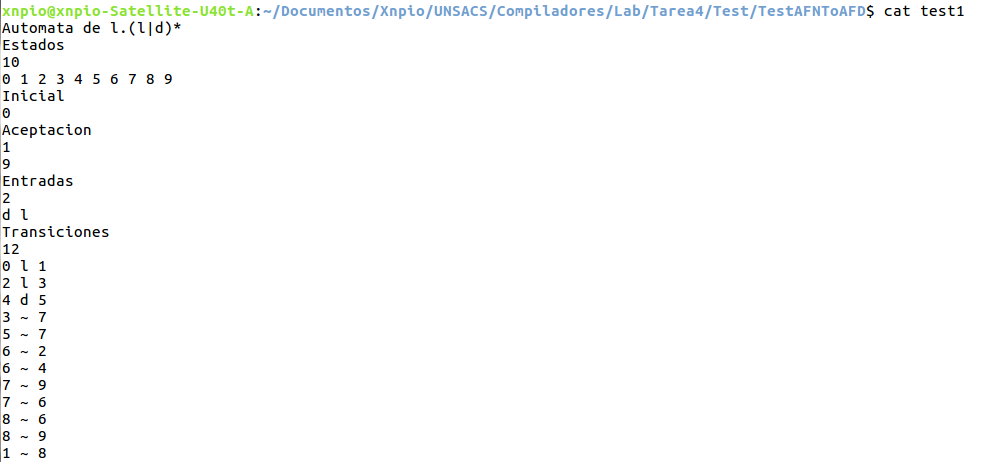
\includegraphics[scale = 0.4]{1.png}
  \caption{Archivo de entrada}
 \end{figure}
 \begin{figure}[H]
  \centering
  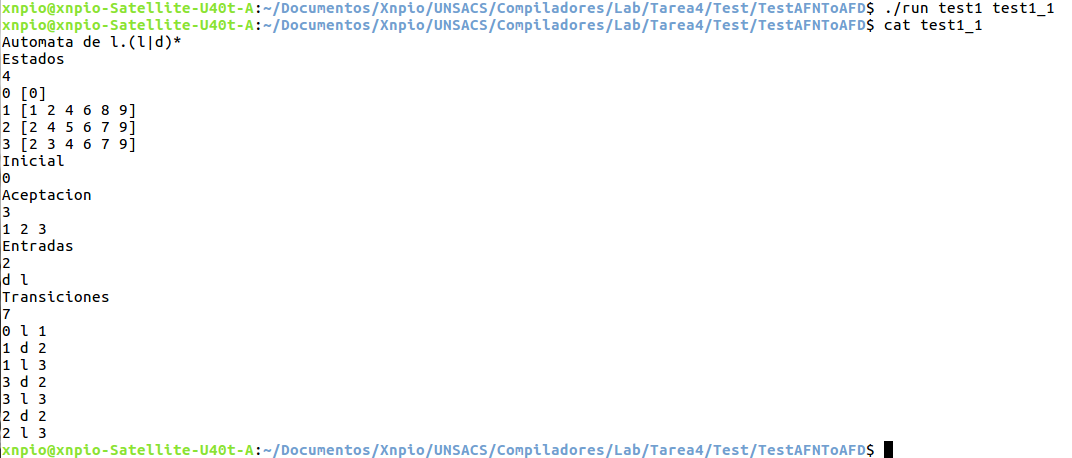
\includegraphics[scale = 0.4]{2.png}
  \caption{Archivo de salida}
 \end{figure}

 \item $(b|bc)^{+}$
 \begin{figure}[H]
  \centering
  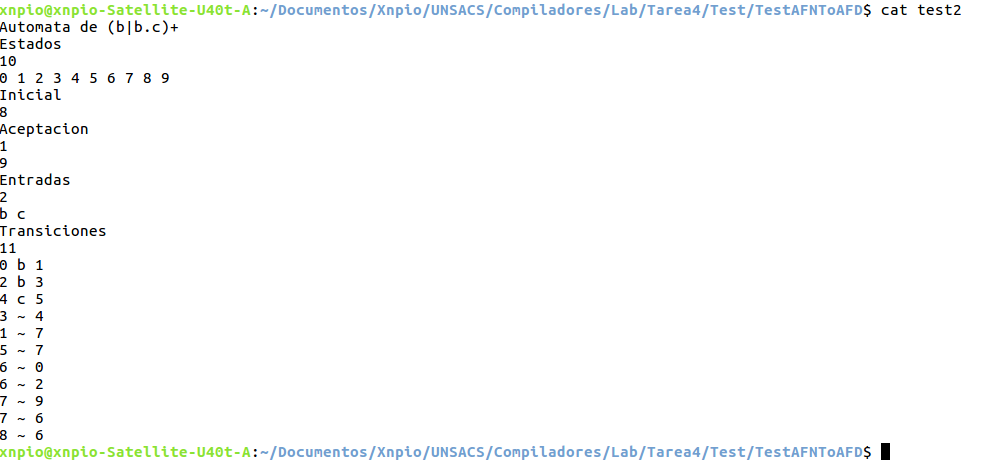
\includegraphics[scale = 0.4]{3.png}
  \caption{Archivo de entrada}
 \end{figure}
 \begin{figure}[H]
  \centering
  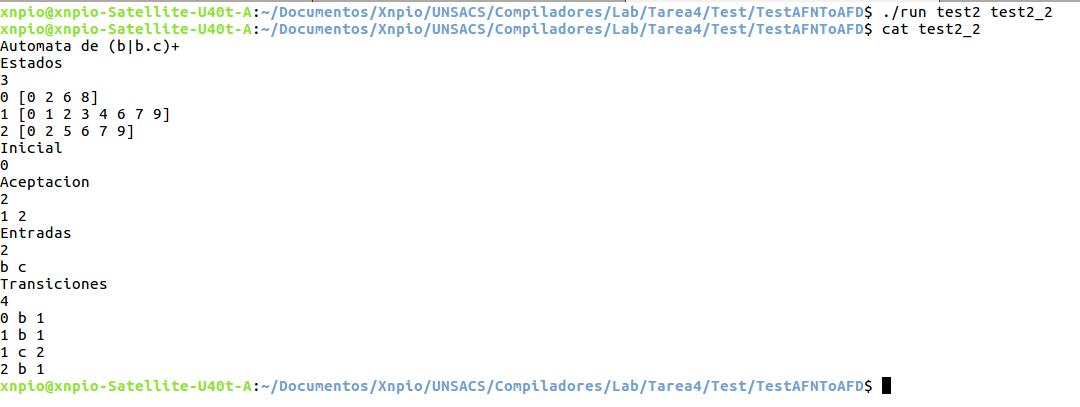
\includegraphics[scale = 0.4]{4.png}
  \caption{Archivo de salida}
 \end{figure}
 
 \item $(abc)*$
 \begin{figure}[H]
  \centering
  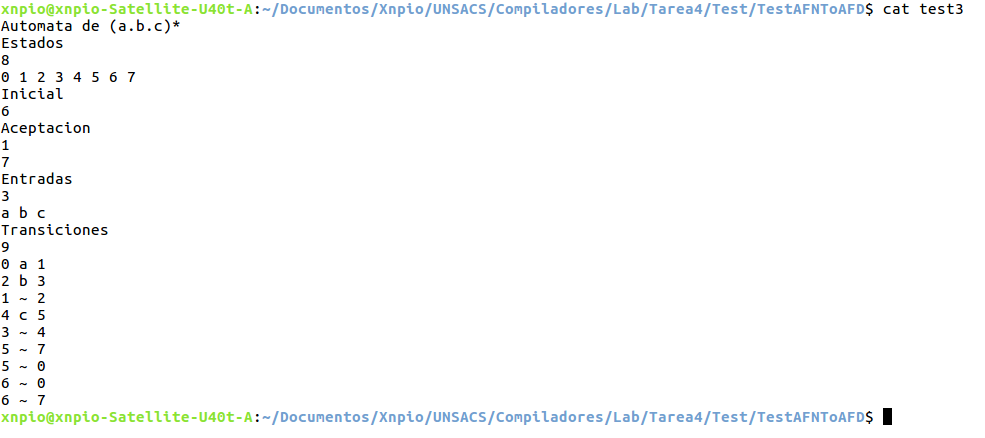
\includegraphics[scale = 0.4]{5.png}
  \caption{Archivo de entrada}
 \end{figure}
 \begin{figure}[H]
  \centering
  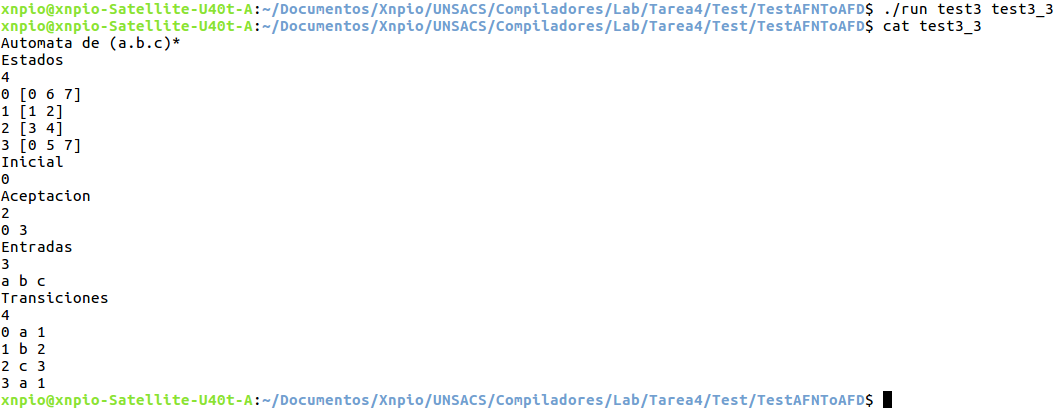
\includegraphics[scale = 0.4]{6.png}
  \caption{Archivo de salida}
 \end{figure}
 
\end{itemize}


 









\end{document}

